\documentclass[border=5pt]{standalone}
\usepackage{tikz}

\usetikzlibrary{
  shapes.geometric,
  backgrounds,
  fit,
  arrows.meta,
  positioning,
}

\tikzset{
  task/.style={
    rectangle,
    rounded corners,
    minimum height=2.5em,
    text centered,
    draw=black,
    fill=blue!15
  },
  isr/.style={
    rectangle,
    rounded corners,
    minimum height=2.5em,
    text centered,
    draw=black,
    fill=red!20
  },
  hw/.style={
    trapezium,
    trapezium left angle=70,
    trapezium right angle=110,
    minimum height=2.5em,
    text centered,
    draw=black,
    fill=gray!30
  },
  callback/.style={
    rectangle,
    dashed,
    minimum height=2.5em,
    text centered,
    draw=black,
    fill=orange!20,
  },
  arrow/.style={
    thick, ->,
    >=stealth,
    opacity=0.5,
  },
  group/.style={
    rectangle,
    rounded corners,
    inner sep=8pt,
  },
}

\begin{document}
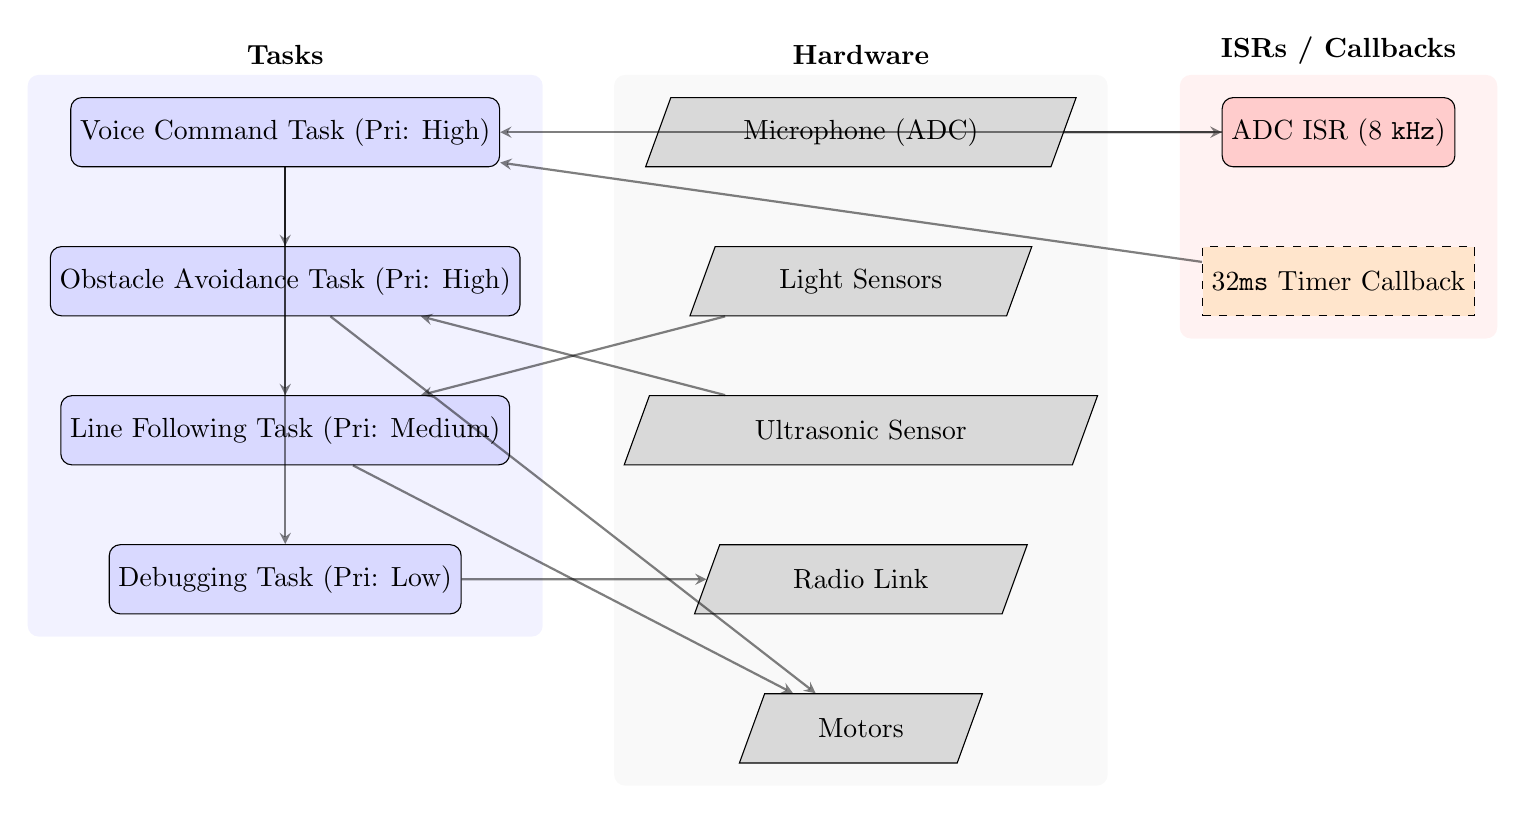
\begin{tikzpicture}[
    node distance=1cm and 2cm,
  ]

  % Hardware blocks
  \node (mic) [hw] {Microphone (ADC)};
  \node (light) [hw, below=of mic] {Light Sensors};
  \node (ultra) [hw, below=of light] {Ultrasonic Sensor};
  \node (radio) [hw, below=of ultra] {Radio Link};
  \node (motor) [hw, below=of radio] {Motors};

  % ISR and callbacks
  \node (adc_isr) [isr, right=of mic] {ADC ISR (8 \texttt{kHz})};
  \node (timer_cb) [callback, below=of adc_isr, yshift=0cm] {32\texttt{ms} Timer Callback};

  % Tasks
  \node (audio_task) [task, left=of mic] {Voice Command Task (Pri: High)};
  \node (obs_task) [task, below=of audio_task] {Obstacle Avoidance Task (Pri: High)};
  \node (line_task) [task, below=of obs_task] {Line Following Task (Pri: Medium)};
  \node (radio_task) [task, below=of line_task] {Debugging Task (Pri: Low)};

  % Groups
  \begin{scope}[on background layer]
    \node[group, fill=gray!5,
    fit=(mic)(light)(ultra)(radio)(motor),
    label=above:{\bf Hardware}] {};
    \node[group, fill=red!5,
    fit=(adc_isr)(timer_cb),
    label=above:{\bf ISRs / Callbacks}] {};
    \node[group, fill=blue!5,
    fit=(audio_task)(line_task)(obs_task)(radio_task),
    label=above:{\bf Tasks}] {};
  \end{scope}

  % Arrows
  \draw [arrow] (mic) -- (adc_isr);
  \draw [arrow] (light) -- (line_task);
  \draw [arrow] (ultra) -- (obs_task);
  \draw [arrow] (audio_task) -- (radio_task);
  \draw [arrow] (line_task) -- (motor);
  \draw [arrow] (obs_task) -- (motor);
  \draw [arrow] (adc_isr) -- (audio_task);
  \draw [arrow] (timer_cb) -- (audio_task);
  \draw [arrow] (radio_task) -- (radio);
  \draw [arrow] (audio_task) -- (line_task);
  \draw [arrow] (audio_task) -- (obs_task);

\end{tikzpicture}
\end{document}
